\section{Problem Formulation}
\label{sec-problem}

%Describe the problem that you are trying to solve, or the application that you
%are trying to implement

Figure \ref{fig:sys-arch} illustrates the general secure memory encryption
architecture used in this study. The threat model assumes that the
on-chip memory, \TT{data-cache}, is secure and tamper-proof whereas the
off-chip memory is not. The \TT{encryption core} between the data-cache is
supposed to provide cryptographic confidentiality properties that prevent
unauthorized principals from reading sensitive information that user's wish to
keep secret.

\begin{figure}[!htb]
  \centering
  \includegraphics[width=0.5\textwidth]{figs/sys-arch}
  \caption{General Memory Encryption Architecture: All on-chip memory accesses,
  between the processor and data-cache, are performed in plaintext whereas all
  off-chip, between the data-cache and DRAM, are encrypted.}
  \label{fig:sys-arch}
\end{figure}

Typically, the encryption core seen in Figure \ref{fig:sys-arch} implements the
\TT{AES-CTR} mode scheme.  Where previous studies have focused on the
performance and area overhead of memory encryption, we wish to explore the
impact of memory encryption on the power consumption of off-chip memory storage
systems. Specifically we want use various computer architecture analysis tools
to simulate memory access traces and model the power overhead of encryption on
DDR4 memory technology. Our first order model characterizes the \TT{ODT} power
overhead when using \TT{Data-Bus Inversion} for realisitic benchmarks
targetting mobile systems using DDR4 memory technology.
